\section{Grundlagen}\label{sec:Grundlagen}
Der Schwerpunkt dieser Arbeit unterteilt sich in zwei Teile, die Signalvorverarbeitung und das \ac{LPC} Verfahren.
Im Folgenden werden die theoretischen Grundlagen für beide Prozesse beschrieben.

\subsection{Signalvorverarbeitung}
Um ein gegebenes Audiosignal einheitlich verarbeiten zu können, muss dieses zunächst mittels verschiedener Verfahren vorbereitet werden.
Ziel dieser Vorverarbeitung ist es, die Effizienz und Effektivität des anschließenden Verarbeitungsprozesses zu erhöhen und somit ein verbessertes Ergebnis zu erzielen \autocite[vgl.][S. 11672]{lokesh_speech_2019}.
Die Vorverarbeitung im Rahmen dieser Arbeit beinhaltet die vier Schritte Rauschreduzierung, Pausen entfernen, Framing und Windowing, welche in den folgenden Unterkapiteln genauer erläutert werden.

\subsubsection{Rauschreduzierung}
Um störende Frequenzen aus dem Audiosignal zu entfernen wird eine Rauschreduzierungsfunktion verwendet.
Die in dieser Arbeit verwendete Funktion nutzt den sogenannten Spectral Noise Gate Algorithmus.
Dabei wird zunächst die Signatur des Rauschens ermittelt.
Basierend darauf kann das Rauschen anschließend verringert werden \autocite[vgl.][S. 25]{kiapuchinski_spectral_2012}.

\subsubsection{Pausen entfernen}
Die für die Sprecherauthentifizierung relevanten Daten stecken in dem aufgezeichneten Signal der Stimme.
Sprechpausen innerhalb des Audiosignals enthalten somit keine brauchbaren Informationen, weshalb diese herausgefiltert werden müssen.
Durch den vorangehenden Schritt der Rauschreduzierung kann hier ein stark vereinfachtes Verfahren gewählt werden.
Liegt das Signal für einen definierten Zeitraum unterhalb einer definierten Lautstärke, werden die entsprechenden Signalwerte aus dem Gesamtsignal entfernt.

\subsubsection{Framing}\label{sec:Framing}
Für eine detaillierte Analyse des Audiosignals muss dieses in kleinere Blöcke unterteilt werden.
Dieser Prozess wird als Framing bezeichnet.
Dabei muss zunächst eine einheitliche Blockgröße festgelegt werden.
Da Stimmsignale aufgrund der Eigenschaften des Vokaltrakts über eine Periode von 10-30 ms stationär sind, wird eine Blockgröße in dieser Zeitordnung verwendet.
Zusätzlich wird eine Überlagerungszeit definiert, welche eine Überlappung der einzelnen Blöcke verursacht.
Durch die Überlappung wird ein Zusammenhang zwischen zwei benachbarten Frames und damit auch den anschließend berechneten Koeffizienten hergestellt \autocite[vgl.][S. 457]{richter_signal_2022}.

\subsubsection{Windowing}
\begin{figure}
  \centering
  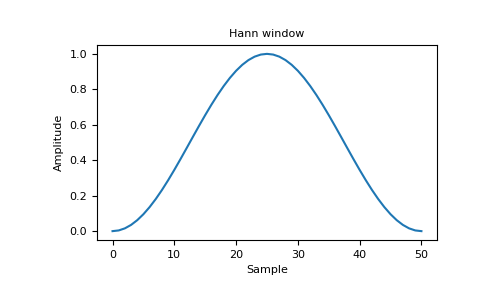
\includegraphics[width=0.8\textwidth, keepaspectratio]{images/hann_window.png}
  \caption{Von Hann Fensterfunktion \autocite{noauthor_numpyhanning_nodate}}
  \label{fig:vonHannFenster}
\end{figure}
Um die bei der Unterteilung des Audiosignals entstandenen Diskontinuitäten aufzulösen, wird eine Fensterfunktion auf die einzelnen Blöcke angewendet.
Abbildung~\ref{fig:vonHannFenster} zeigt die von Hann Fensterfunktion, welche neben dem Hamming Fenster zu den typischen Fensterfunktionen in der Audiosignalverarbeitung zählt.
Durch den Nulldurchgang am Anfang und Ende der Fensterfunktion werden die Amplituden des Blocksignals nach Anwenden der Funktion an den Grenzen auf Null gezogen, wodurch sich ein kontinuierlicher, periodischer Signalverlauf ergibt \autocite[vgl.][S. 462]{richter_signal_2022}.

Wird der Schritt des Windowing nicht durchgeführt, führt dies zu einem Phänomen namens Spectral leakage.
Bei der Transformation des Signals von dem Zeitbereich in den Frequenzbereich, resultiert der Amplitudensprung an den Blockenden in der Registrierung einer vielzahl von Frequenzen.
Wie der Name bereits beschreibt, wird aus einer eindeutigen Frequenz, ein Spektrum aus Frequenzen, die nicht Teil des Signals sind \autocite[vgl.][S. 1296]{wu_new_2012}.
% TODO: Bessere Quelle finden

\subsection{Linear Predictive Coding Koeffizientenberechnung}
Ausgehend von dem in Frames unterteilten Audiosignal, müssen nun für jeden Frame \ac{LPC} Koeffizienten berechnet werden, welche anschließend für die Zuordnung des Audiosignals zu einer spezifischen Stimme genutzt werden können.
Die Grundlage von \ac{LPC} bildet das \ac{AR} Modell, welches zunächst beschrieben wird.
Anschließend wird der theoretische Zusammenhang zwischen \ac{AR}, \ac{LPC} und der menschlichen Stimme dargestellt.

\subsubsection{Autoregression Modell}
Die \ac{AR} basiert auf dem Konzept der multiplen Regression und wird auf zeitlich veränderliche Prozesse angewandt.
Dabei wird eine Kriteriumsvariable unter Betrachtung von n Prädiktorvariablen vorhergesagt \autocite[vgl.][S. 37-38]{canela_multiple_2019}.
Im Speziellen Fall der \ac{AR}, handelt es sich bei den Prädiktorvariablen um vorhergehende Werte des Prozesses.
Ein \ac{AR} Modell sagt somit den Wert zu einem Zeitpunkt $n$, basierend auf $p$ Vorgängerwerten des Prozesses voraus.
Es gilt somit der in Formel~\ref{eq:autoregression} dargestellte Zusammenhang, wobei $\hat{s}_n$ den vorausgesagten Wert, $s_{n-k}$ die vorhergehenden Werte, $a_{k}$ die Regressionsgewichte und $p$ die Anzahl an verwendeten Vorgängerwerten darstellt \autocite[][S. 1304]{atal_effectiveness_1974}.
\begin{equation}
  \hat{s}_{n} = \sum_{k=1}^{p} s_{n-k}a_{k}
  \label{eq:autoregression}
\end{equation}

Zur Bestimmung der Regressionsgewichte wurden verschiedene rekursive Verfahren entwickelt.
Neben der Yule-Walker Methode stellt der Burg Algorithmus eine beliebte Alternative dar, welcher in \citeauthor[][S. 443]{marple_new_1980} beschrieben ist.
% Evtl: Formeln des Burg Algorithmus auflisten und erklären
% Evtl: Was hat Yule-Walker und Levinson damit zu tun?

\subsubsection{Linear Predictive Coding}
Wie bereits zu Beginn der Arbeit erwähnt, wird bei dem Verfahren \ac{LPC} der Ansatz verfolgt, Rückschlüsse von dem akustischen Signal auf die Stimmerzeugung zu ziehen.
Dazu wird ein \ac{AR} Filter verwendet um ein vereinfachtes Modell des menschlichen Stimmtrakts zu erstellen.
Die Regressionsgewichte $a_k$ entsprechen dabei den \ac{LPC} Koeffizienten.
\newline
\newline
Bei der Stimmerzeugung spielen die sogenannten Formanten eine Rolle.
Diese beschreiben die akustische Energie in einem unveränderlichen Frequenzbereich, welche wiederum von den Resonanz- und Interferenzeigenschaften des Artikulationsraums abhängen.
Dadurch werden bestimmte Frequenzen verstärkt, während andere gedämpft werden \autocite[vgl.][S. 259]{fitch_evolution_2000}.
Das durch die \ac{LPC} Koeffizienten erstellte Modell erfasst die Resonanzeigenschaften des Signals, wodurch Rückschlüsse auf die Formanten geschlossen werden können.
Da die Struktur der Formanten Sprecherspezifisch ist, kann der Sprecher somit über die \ac{LPC} Koeffizienten identifiziert werden \autocite[vgl.][S. 117]{sidorov_text-independent_2010}.
\newline
\newline
Zur Berechnung der \ac{LPC} Koeffizienten wird zunächst die selbe Annahme wie in Kapitel~\ref{sec:Framing} getroffen, dass sich die Form des Vokaltrakts und das in den Stimmritzen erzeuge Signal über den betrachteten Zeitraum nicht verändert \autocite[vgl.][S. 1304]{atal_effectiveness_1974}.
Somit lassen sich die Koeffizienten des \ac{AR} Filters mittels des Burg Algorithmus berechnen.